\documentclass[11pt]{sdm}

\usepackage{graphicx}
\graphicspath{{../img/}}

\usepackage{subcaption}
\usepackage{cleveref}
\usepackage{comment}
\pagestyle{plain}

\usepackage{hyperref}
\usepackage{url} \urlstyle{sf}
\newcommand{\email}[1]{\href{mailto:#1}{#1}}

\usepackage{xspace}

\usepackage[dvipsnames]{xcolor}
\newcommand{\addref}[1]{\colorbox{TealBlue!100}{\textcolor{white}{\textbf{$[$\ifx&#1&\ \else#1\fi$]$}}}}
\newcommand{\todo}[1]{\colorbox{Red!75}{\textcolor{white}{\textbf{TODO\ifx&#1&\else: #1\fi}}}}
\newcommand{\done}{\colorbox{YellowGreen!100}{\textcolor{white}{\textbf{DONE}}}}
\newcommand{\review}{\colorbox{YellowOrange!100}{\textcolor{white}{\textbf{REVIEW}}}}

\newcommand{\dspot}{DSpot\xspace}
\newcommand{\pitest}{Pitest\xspace}
\newcommand{\evosuite}{EvoSuite\xspace}

\usepackage{listings}
\lstset{%
%  backgroundcolor=\color{white},   % choose the background color; you must add \usepackage{color} or \usepackage{xcolor}
  basicstyle=\small,        % the size of the fonts that are used for the code
  captionpos=b,                    % sets the caption-position to bottom
  commentstyle=\color{cyan},    % comment style
  escapeinside={(*@}{@*)},          % if you want to add LaTeX within your code
  keywordstyle=\color{blue},       % keyword style
  stringstyle=\color{red},       % keyword style
  numberstyle=\tiny\color{black}, % the style that is used for the line-numbers
  stepnumber=1,                    % the step between two line-numbers. If it's 1, each line will be numbered
  title=\lstname,                   % show the filename of files included with \lstinputlisting; also try caption instead of title
  language=Java,
  breakatwhitespace=false,         % sets if automatic breaks should only happen at whitespace
  breaklines=true,                 % sets automatic line breaking
  extendedchars=true,              % lets you use non-ASCII characters; for 8-bits encodings only, does not work with UTF-8
  %frame=single,                    % adds a frame around the code
  showspaces=false,                % show spaces everywhere adding particular underscores; it overrides 'showstringspaces'
  showstringspaces=false,          % underline spaces within strings only
  showtabs=false,                  % show tabs within strings adding particular underscores
  tabsize=2                       % sets default tabsize to 2 spaces
}

\usepackage{ragged2e}

\title{Search-Based Test Amplification}

\author{Simon \textsc{Bihel}}
\supervisorOne{Benoit \textsc{Baudry}}
\supervisorTwo{~}
\team{KTH Royal Institute of Technology}
\school{ens-Rennes}

\domain{Domain: Software Engineering - Artificial Intelligence}

\abstract{%
  \justify{%
% ----- Context
With practices such a test-driven development, software projects now come with strong test suites.
They embed knowledge of supported inputs and expected behavior which make it easy to detect bugs such as unwanted changes in behavior as the code evolves with time.
But writing and maintaining a large number of test cases is time consuming for the developers and as they are humans they can miss some edge cases resulting in sub-optimal testing.
% ----- SBST
To address these problems, automated methods have been developed to generate tests from scratch, optimize test suites, or extend test suites.
Because the space of possible tests is so vast, approximate meta-heuristic methods are often used for these problems.
In particular, evolutionary methods are particularly suited for amplifying and improving an existing test suite by generating variants of test cases.
% -----
Tools have been developed to amplify test suites but optimizing the generated tests is still an open problem.
Because developers are still involved in the loop, by reviewing and merging new tests, this thesis focuses on reduce the amount of work the developer has to provide by reducing the number of generated tests and making them easier to understand for a human.
  }
}

\date{February 2018}

% Ought to be 10 to 15 pages long

\begin{document}
\maketitle

\section*{Introduction}
\label{intro}
The adoption of test-driven and agile methods for software development and with the more recent emergence of DevOps, developers have serious incentives to write strong test suites.
They contain large number of test cases, which embed rich knowledge about relevant input and expected behavior.
The key incentive for developers is that these test suites can be automatically executed on demand to minimize regression bugs as the code continuously evolves.
However, the production and maintenance of large test suites to detect these regressions is time consuming, and, consequently, developers tend to focus on nominal paths when writing test cases, missing the corner, rare cases.
The key challenge we address in this thesis is as follows: automatically analyze existing test cases and exploit the knowledge that developers have embedded there in order to generate variant test cases that target new behavior.
This is called \emph{test amplification}~\cite{danglot2017emerging}.

Automatic test generation is a traditional area in software testing~\cite{mcminn2011search}: the goal is to generate test cases according to a specific test criterion.
However, test generation techniques tend to ignore the existence of manually written test suites: they assume that no tests exist at all, or that they are either too few or of too low quality for being considered useful in the generation process.
The emerging field of test amplification considers a different approach and explicitly aims at exploiting knowledge from existing test cases.
For this thesis, we focus on search-based techniques to exploit this knowledge.

Search-based software engineering~\cite{harman2001search} is the discipline that investigates meta-heuristic search (e.g., genetic algorithms or simulated annealing) to automate software engineering tasks.
In the case of automatic test generation, this consists in iteratively generating test cases and selecting the ones that improve an objective, expressed as a fitness function (e.g., increase code coverage).
This thesis investigates meta-heuristics to optimize the process of unit test amplification.
For example, test amplification tends to generate a large number of new test cases.
This is challenging for the developers who wish to minimize the time spent on test execution and who want to understand these new tests before integrating them in their code base.
Meta-heuristics can serve to minimize the number of relevant test cases, or generate summaries for developers to understand the new test cases.

Search-based test amplification is an experimental approach to software research.
The thesis will hence contain a significant experimental part, which consists in testing the meta-heuristics on real-world open source projects and determine the relevance of the search-based technique for amplification.
The search-based algorithms will be included in the~\dspot{}~\cite{baudry2015dspot} tool for experimental purposes.

% ----- Outline
After explaining the basics of Search-Based Software Testing in Section~\ref{sbse} we will present how it can be used to amplify test suites in Section~\ref{tsa}.
In Section~\ref{planned} we detail the different paths the internship could explore.


% ========== Section 1 ==========
\section{Search-Based Software Engineering}
\label{sbse}

In this section we present the reasons for the emergence of Search-Based Software Engineering (SBSE)~\cite{harman2001search,mcminn2011search} and give examples of applications.

\subsection{Motivations}
\label{motiv}
% ----- History
In the field of mathematical optimization, meta-heuristic techniques have been developed.
With the use of specific strategies, such methods can find sufficiently good solutions to optimization problems in a lower time than would be required to find an optimal solution.
They are especially useful in situations with incomplete information and often rely on randomness to explore the \textit{search space} (i.e.\ the set of possible solutions).

% ----- Complexity of problems in SE
With the rise of complexity in software projects, needs for automation and approximation rose.
In optimization problems where it is impossible to predict the performance of a configuration and where too many configurations are available to try, approximate methods started to be used.
In the field of software testing, which is often a tedious job for developers, approximate tools started to be built in order to write tests in place of a human.

% ----- Announcing SBSE
This use of meta-heuristic techniques to solve software engineering problems is what constitute the field of Search-Based Software Engineering (SBSE).
The formulation of SE problems as optimization is at the heart of all works of SBSE as we need to define a function to maximise for goals that are not always easy to formally describe, and we need to define the search space with what actions (i.e.\ manipulations) can the meta-heuristic algorithm employ.

\subsection{Search-Based Optimization Algorithms}
\label{example_algo}
To reach a software engineering goal for these complex systems we use \textit{soft-computing} (or \textit{computational intelligence}) to find inexact or sub-optimal solutions in a reasonable time.
In Section~\ref{basic_algo} we present some algorithms to give an idea of the capabilities of these techniques.
In Section~\ref{fitness_func} we show how we can pursue engineering goals with these optimization processes.

\subsubsection{Basic algorithms}
\label{basic_algo}

\begin{figure}
  \centering
  \begin{subfigure}[b]{0.33\textwidth}
    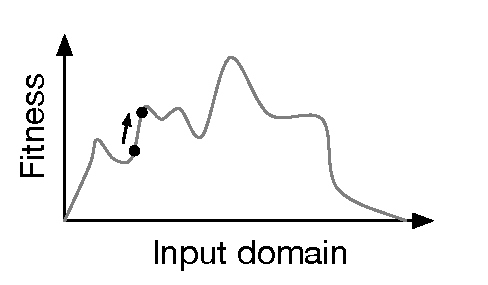
\includegraphics[width=\textwidth]{hillclimbing}
\caption{Hill Climbing}
\label{fig:hill_climbing}
  \end{subfigure}%
~%
  \begin{subfigure}[b]{0.33\textwidth}
    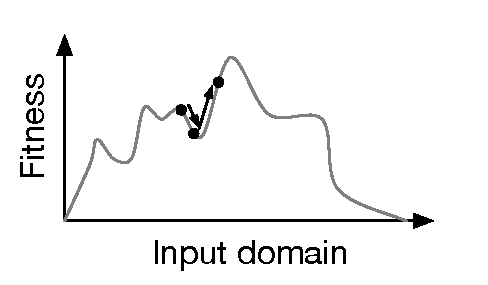
\includegraphics[width=\textwidth]{simulated_annealing}
\caption{Simulated Annealing}
\label{fig:simulated_annealing}
  \end{subfigure}%
~%
  \begin{subfigure}[b]{0.33\textwidth}
    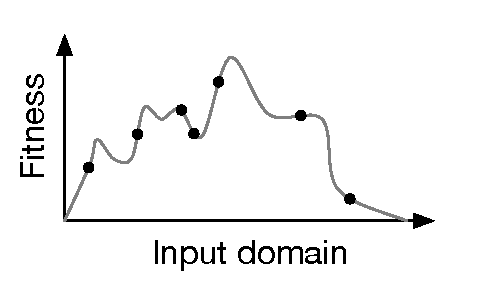
\includegraphics[width=\textwidth]{genetic_algo}
\caption{Genetic Algorithm}
\label{fig:genetic_algo}
  \end{subfigure}
\caption{Basic optimization algorithms}
\label{fig:optimization_algos}
\end{figure}

% ----- Hill Climbing & Simulated Annealing
The simplest form of such algorithm is the Hill Climbing.
Its process is pictured in \figurename~\ref{fig:hill_climbing}.
It only consists of starting from a random position and from there, and iteratively, find a direction to move in to improve the fitness function.
As the algorithm is searching only for direct improvement we can only find a local optima.
We could start the algorithm with a different starting position but we can also allow the algorithm to move in a direction that does not improve directly the score in the hope to later find a higher local optima.
This is called Simulated Annealing and we show an example in \figurename~\ref{fig:simulated_annealing}.

% ----- Genetic Algorithm
These methods are described as `local' search approaches as they only consider only one solution at a time.
Genetic Algorithms (GAs), on the other hand, consider multiple points in the search space at once as shown in \figurename~\ref{fig:genetic_algo}.
Each point is referred as an `individual' and the set of individuals is called a `population'.
Each iteration we keep the fittest individuals and do crossover of them to generate new individuals.
In a multi-dimensional search space we can see dimensions as genes and a crossover is the combination of genes from two individuals.

% ----- How to use them for real problems?
In order to use these methods for software engineering problems we have two requirements:
\begin{description}
  \item[Representation] We need to encode our individuals, e.g.\ programs, in a way that they can be manipulated by the optimization algorithm. We will explore this problem in Section~\ref{applications}.
  \item[Fitness function] We need a way to tell that an individual is better than another one, e.g.\ that a program is safer than another one. We present the use of software metrics as fitness function next in Section~\ref{fitness_func}.
\end{description}

\subsubsection{Metrics as fitness functions}
\label{fitness_func}
% ----- Motivations for metrics
Evaluating a piece of code automatically is not an easy task depending on the property we want to assess.
To evaluate the performances, one might just run the program with a certain kind of workload.
But when we want to tell the chances of having bugs or tell that the modularity will not get in the way of future evolution, it gets harder.
These properties are already difficult to express informally and often depend on a programmer's intuition that has developed over years of practice.
Because companies need to be able to tell if their products are of good quality, significant efforts from the industry and research worlds have been put in developing \textit{metrics}.

% ----- Metrics for testing
As the internship will focus on testing, we will spend a bit of time here to present metrics used to assess the quality and quantity of testing, and thus the likelihood of absence of bugs.
One that is widely used is the \textit{code coverage} metric.
Informally, it is the amount of code executed by a test suite.
It can be as simple as the percentage of statement executed, or something more complex and thus more likely to find edge cases and bugs.
For example, the branch coverage, where you want every branch of each control structure to be executed.
Many variants exist, each with its bugs category that it can find and its cost as it requires the execution of many tests.

% ----- Mutation score
To add more confidence that the test suite is effective, we can evaluate it by voluntarily introducing bugs in the software and see if it is capable of detecting them.
This is what we call \textit{mutation testing} as we are creating \textit{mutants} of the main piece of software.
In Section~\ref{applications} we explain how to create software mutants.

\subsection{Genetic Improvement}
\label{applications}
% ----- Intro to genetic improvement
SBSE techniques can be applied to modify and improve existing software in what is called \textit{Genetic Improvement} (GI)~\cite{petke2017genetic}.
In order to modify a program we need a representation and \textit{operators} (i.e.\ set of possible actions).
Numerous representations exist such as ASTs, bytecode, the program's text file itself, etc.
Then the operators can range from modifying elementary operators (e.g.\ addition) to deleting unused part of the program.

% ----- Why is it possible?
The range of possible programs is vast but GI is a reasonable approach.
We are not generating programs from scratch so we have a strong starting population for evolutionary algorithms.
Industry-level code is repetitive, so even with a simple set of operators we can change the behavior of a program and still being valid.
In the case of software projects with a test suite, we can use it as a guide for semantic faithfulness while trying to improve another metric.


% ========== Section 2 ==========
\section{Test Suite Amplification}
\label{tsa}
In this section we present the specific problem of enhancing an existing test suite~\cite{danglot2017emerging}.
First, Section~\ref{motiv_tsa} exposes the motivations for trying to amplify a preexisting and seemingly strong test suite.
Then Section~\ref{related} presents a few papers to give an idea of the related works.
The tool that the internship will be based on is called \dspot{} and it is presented in Section~\ref{testsuite_eval}.

% TODO \addref{new survey paper}

\subsection{Motivations}
\label{motiv_tsa}

\begin{lstlisting}[caption={An archetypal example of an object-oriented test case  (taken from the Apache Commons Collections, in the class TreeListTest, line 270)},label=lst:archetype,float,language=java,numbers=left]
testIterationOrder() {
  TreeList tl = new TreeList(10); (*@\label{input-begin}@*)
  for (int i = 0; i < size; i++)
    {tl.add(i);}(*@\label{input-end}@*)
  int i = 0;
  ListIterator it = tl.listIterator();(*@\label{test}@*)
  while (it.hasNext()) {
    Integer val = it.next();
    assertEquals(i++, val.intValue());
  }
}
\end{lstlisting}

% ----- Tests
An example of Java test case is given in Listing~\ref{lst:archetype}.
We can see that it triggers the System Under Test with inputs and then assert that certain properties hold.
Tests assess the quality of a software by evaluating some situations.

% ----- Why it is possible
Important projects from big companies now come with extensive test suites thanks to good practices.
It is thus reasonable to try and see if we can push even further the quality of such projects.
To achieve that, we want automated tools that can generate additional tests in order to evaluate more situations, or rework the test suite to have a better score for a certain fitness function (e.g.\ optimizing tests execution time).
% In either way we preserve the original, hand-written, test suite as it contains much of the human knowledge of the expected behavior of the software.

% ----- How we can use the test suite
We can simply use GI on the test suite to improve it as you would for any kind of piece of code.
But more importantly, we can see the test suite as a set of specifications that gives us knowledge about what the software is supposed to do --- it is called an \textit{oracle}.
So we have a relation between the software and its test suite and we can use this relation to extend both, for example a bigger and more precise oracle.


\subsection{Related Works}
\label{related}
Before presenting the tool that the internship will focus on, we present some related works to give an idea of amplification goals and amplification techniques.
In Section~\ref{brefactoring} we present a tool with the goal of helping fault-localization.
Then two other general purpose test data generators are presented in Sections~\ref{tdr} and~\ref{evosuite}.

\subsubsection{B-Refactoring}
\label{brefactoring}
% ----- Introduction
To give an example of a precise software engineering goal and test suite refactoring, we chose to present B-Refactoring~\cite{xuan2016b}.
It is a test code refactoring technique to split a test case into small test fragments, helping for fault localization for example.

% ----- Precise goal
To explain in more details, the goal is to have a simpler part of the control flow for each test.
Test cases, especially hand-written ones, can test different properties at once but the problem is that certain analysis which use tests traces require simple control flows in order to increase their precision.
An example is the process of bug fixing, in which you need to locate the source of the bug in order to fix it.
A test suite based tool for fault localization would run the test suite and, using the test traces, locate the faulty part that is executed by the failed tests and not by the passing tests.
In the case of an \texttt{if} condition where in the execution of a test where both branches are executed, there is not enough precision for the fault localization tool to be effective.

% ----- How to they do it?
To have a test suite that is better suited for fault localization, B-Refactoring will \textit{split} tests that explore multiple branches into smaller tests --- keeping the same overall behavior.
The split is done by splitting statements of the test case, resulting in smaller tests that possibly aren't \textit{impure} (i.e.\ explore a single branch of the control flow).
To form the groups of statements, the tool goes through the statements until one that causes the execution of two branches of the control flow, closes the current group and continues with a new empty group.

\subsubsection{Test Data Regeneration}
\label{tdr}
% ----- Introduction
An example of work on generating additional test cases from an existing test suite is the work of Search-based Test Data Regeneration (TDR)~\cite{yoo2012test}.
It is a general-purpose technique that modifies (i.e.\ \emph{regenerate}) test cases to improve the fault detection capability of a test suite.
A modified test case should keep the \emph{same behavior} according to a certain metric (i.e.\ it has the same contribution to test objectives).
Having more tests with different inputs brings redundancy which can be desirable for more robustness, and it brings more diversity as hand-written test can miss some cases.
It is useful to avoid the system to be over-fitted to the test suite (i.e.\ it knows the expected output of a test in advance).

% ----- How do they do it?
The TDR technique is based on the hill climbing algorithm with the notions of neighbour solutions and search radius.
If we look at the integer input domain, modification operators will try to generate neighbour values.
Integer operators are $\lambda x.x + 1$, $\lambda x.x - 1$, $\lambda x.x * 2$, and $\lambda x.\lceil x / 2\rceil$ and they generate inputs that are shifted of scaled.
To control the search process, a limit is set on the number and size of modifications that can be applied on the input vector.
Among neighbours tests, among the ones that have the same quality metric as the original, the most different one is kept.

Aiming for different inputs with identical behaviour is a difficult problem and induces the generation of many non-viable tests.

\subsubsection{EvoSuite}
\label{evosuite}
% ----- Introduction
\evosuite{}~\cite{fraser2011evosuite} is a state-of-the-art and industry-grade Java tool that can generate test suites from scratch using a search-based approach.
Instead of studying each test case independently,~\evosuite{} manipulates whole test suites, seeing them as an individual whose genes are test cases.
In this case tests are sequences of method calls exercising the unit under test and setting up complex objects in order to do so.
Multiple metrics can be used as fitness function of a test suite, for example code coverage or mutation score.

% ----- Assertion generation
Assertions are also generated automatically.
They are there to increase the mutation score, so the test cases will be executed on several mutants of the main software piece and assertions will be added to detects these mutants (i.e.\ increase regression detection).
This method generates many assertions and has a risk of over-fitting so~\evosuite{} tries to reduce the set of assertions.
And while it is sufficient for regression testing, it is difficult to build an oracle capable of knowing what the software is really supposed to do as opposed to what it can do with its current version.

At the end of the process, developers have to review and accept the tests.
Automatically generating tests from scratch that a developer can understand is very difficult because the tool sees a fitness score while the developer searches for a logical setup, meaningful triggers and relevant assertions.


\subsection{DSpot}
\label{testsuite_eval}

\subsubsection{Introduction}
\begin{figure}
  \centering
  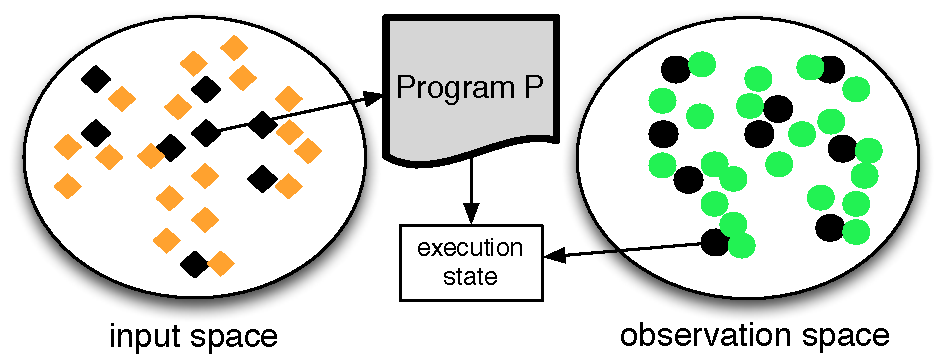
\includegraphics[scale=0.5]{io-spaces.pdf}
  \caption{On the left, the testing input space is composed by specified input points (orange diamonds) and unspecified input points (black diamonds). On the right, the observation space over a given program state depicts the assertions of tests. The green circles are values that are already asserted in the existing test suite, the newly added assertions are shown as black circles.}
\label{fig:io-spaces}
\end{figure}

\begin{figure}
  \centering
  \fbox{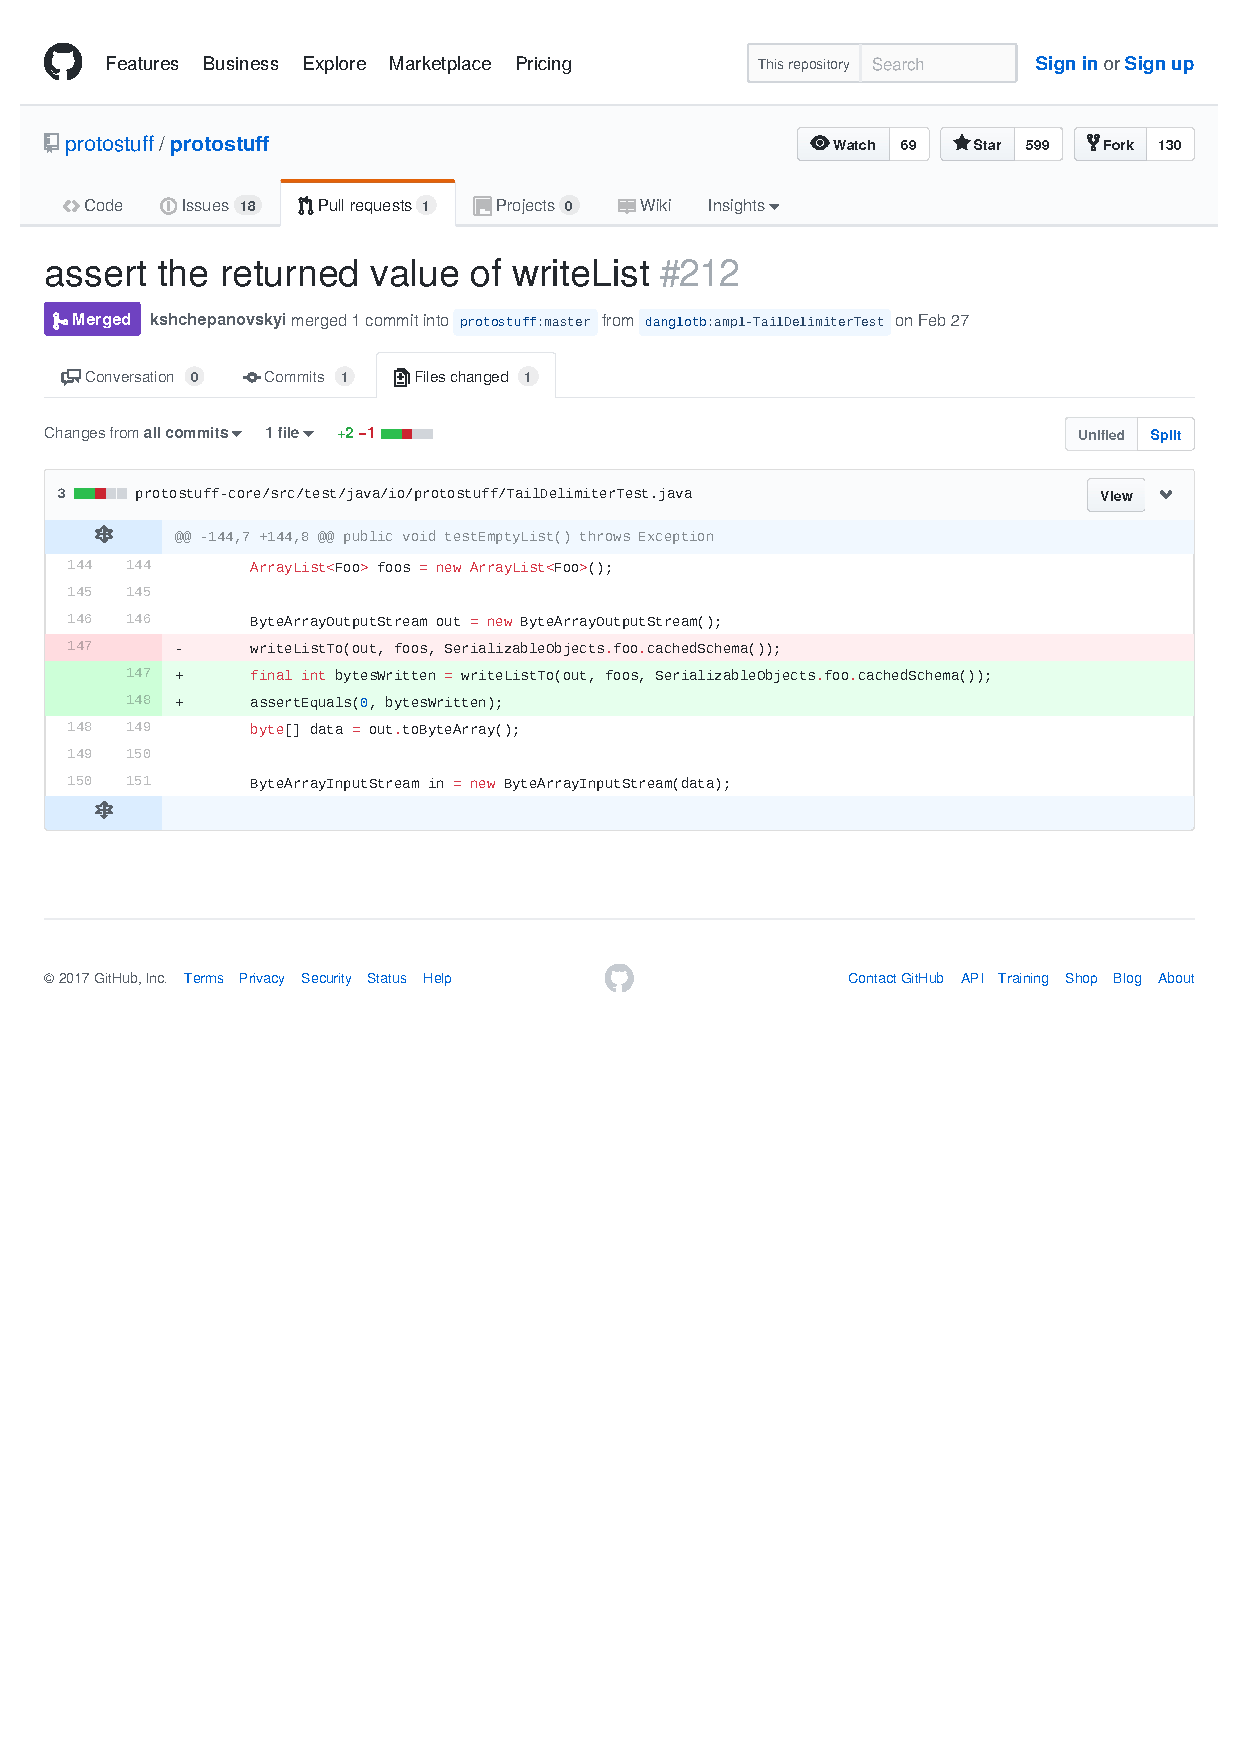
\includegraphics[trim=2cm 17.02cm 4.09cm 10.46cm, clip]{rq3_resources/protostuff.pdf}}
  \caption{Example of what \dspot{} produces: a diff to improve an existing test case.}
\label{fig:diff-protostuff}
\end{figure}

% ----- Introduction
In previous work, we have seen techniques used to enhance a test suite without the input of humans.
This induces limitations, for example we might only optimize a test suite while keeping the same set of behaviors triggered, or new tests can only detect obvious bugs such as crashes, or new tests are there only to detect regression.
With~\dspot{}\footnote{\url{https://github.com/STAMP-project/dspot}}~\cite{baudry2015dspot} the goal is to extend the oracle by covering more of the input space ---~\figurename~\ref{fig:io-spaces} illustrates the input and output spaces of test cases.
% TODO \addref{new dspot paper}
It is a Java tool that tries to improve the mutation score of the test suite.
The tool generates mutants of the software and if the test suite does not detect these changes, adds a test case or improves an existing test case that will check the appropriate part of the software.
This new test is submitted to the developers for them to decide whether to keep it or not.
An example of such pull-request is shown in~\figurename~\ref{fig:diff-protostuff}.

% ----- Programmer's input
The new tests can detect changes in behavior that are not detected by the current test suite.
We cannot assume that the current software version, if it passes all tests, is perfect.
This is why we need to ask the programmer, whether the current behavior is correct and whether they think the generated test is good.
In other words when we found changes to are undetected, we have reached the limits of the oracle and ask the programmer to validate the proposed extension.

\subsubsection{Inner Workings}
\dspot{} has two kind of amplifications, one for generating new inputs and one for generating new assertions.
Next we present them and also give some hints on the implementation.

\paragraph{I-Amplification}
To generate new test inputs from existing test~\dspot{} uses different operators.
\begin{description}
  \item[\textit{Amplification of literals}] Similarly to TDR (Section~\ref{tdr}) literals (numeric, boolean, string) are replaced by neighbours. For example, an integer can be multiplied by 2 or a random character can be added to a string.
  \item[\textit{Amplification of method calls}] Methods calls can be duplicated, removed, or made-up by picking a random variable in the test and calling one of its methods with random parameters.
  \item[\textit{Test objects}] If a new object is required for an amplified method call, one of the appropriate type will be built by using the default constructor.
\end{description}

\paragraph{A-Amplification}
To extend the oracle~\dspot{} adds assertions in tests in a similar fashion to~\evosuite{} (Section~\ref{evosuite}).
Assertions are added on objects from the original test case.
They are generated as follows: the state of program is collected after execution of the test case to know the actual values and use these values as oracle.

Because tests are improved versions of manually written tests, the assertions are of better quality but also easier to understand for the developers.

\paragraph{Implementation}
\dspot{} is written in Java, uses Spoon~\cite{pawlak2016spoon} for analysis and transformation of tests, and uses Pitest\footnote{\url{http://pitest.org/}} to measure the mutation score.

Because the assertions and their expected values are hardcoded we do not want tests with non-deterministic executions.
In order to avoid generating such tests each new test is executed multiple times and if it fails at least once then the test is rejected.
It does not give guarantee on the absence of non-deterministic but it can remove obvious ones and ease the review process of developers.


% ========== Section 3 ==========
\section{Planned Work}
\label{planned}
This section explains the different paths that we could explore during the internship.

\subsection{Evaluation of the Added Value of Hand-Written Tests}
\label{evaluation}
% ----- Motivations
Up to now, no empirical evaluation has been done on the added value of amplification rather than generating tests from scratch.
Even if it seems obvious that it helps, with insights on the semantics and a strong starting population for evolutionary algorithms, it is important to experimentally measure the gain.

% ----- Methodology

\subsection{Using Literals Found in Source Code}
\label{mutation}
% ----- Problem statement
Among elementary types are character strings.
With a problem such as test data generation, it is often difficult to generate valid strings as the search space is large and specific values are expected.
But in such cases where there are explicit equality tests, one could collect these precise values and limit the search space to them.

% ----- How could we do it?
We have different options to achieve this collection.
A purely dynamic of doing things would be to instrument the code to detect when the argument is used in an equality test and from there collect a value that would be accepted.
Another possibility would be to statically harvest all literals found in the code.

% ----- How would we evaluate it?
As an evaluation, a comparison with and without this enhancement on programs that heavily rely on string would be sufficient.

\subsection{Creating mutation operators for specific data structures}
\label{create_operators}
% ----- Problem statement
In the same branch of the strings generation problem, with complex and multi-dimensional data structures that often need precise comfiguration, we need smarter generator and mutation operators to avoid senseless inputs.

\subsection{Stacking mutations}
\label{stacking}
% ----- Problem statement
For now in~\dspot{}, when a program is modified, a single mutation operator is applied.
It makes it easy to detect precise weaknesses in the System Under Test by at the same time we could detect more weaknesses by stacking mutations.
Evolved tests would be more complex and more distant from the existing test suite.

% ----- Contribution
Of course there would be smaller chances of generate good inputs but we could study the interactions between various mutation operators to only use the ones that would work well together.

\subsection{Explanations and Importance}
\label{explanation}
% ----- Problem statement
When a new test is generated and found useful, a merge/pull request is created for the developer to decide whether to accept the new test.
The role of the developer is to judge the usefulness of the additional test.
As always we want to minimize to efforts from the human so we need to help the developer by explaining the new test.
It is also essential to explain why a test is relevant because in most cases a test that is not understood will be at best ignored, at worst labeled as false positive~\cite{bessey2010few}.

A similar problem is the ordering of pull requests.
If we could in some way define the importance of tests, we could present to the developer the most important tests first.
The importance could be based on the amount of regression bugs the test could detect (the highest mutation score) but this could lead to prioritize long and complex tests.

In the end the two problems are linked because we want tests that focus on one particular scenario so it is simple and easier to understand for the developer and also we want to understand the real value of this scenario to be able to provide an explanation.

\subsection{Learning the set of good amplification operators}
\label{learning}
% ----- Problem statement
In order to generate the least amount of programs that don't make sense, knowing which operators work well in general would make them used more often.

\subsection{Reduce the amplified tests to a minimal set of useful tests}
\label{minimal}
% ----- Problem statement
Overall, the ultimate goal would be to generate a minimal set of amplified tests.

% ----- How would we do it?
In order to achieve this, we could explore different options.
With a post treatment we would, from a complete set of tests, we could remove overlapping tests, fusion others, split tests depending on the different goals achieved, etc.
On the other hand, to avoid tests that would end up being removed or modified we could generating from the start with a more detailed goal.
In this way would could also replace another test if needed.


\section*{Conclusion}
\label{conclu}
In this document we have presented the use of approximate techniques in order to reach software engineering goals.
In particular we have explore the field of test suite amplification which aims at increasing the quality of a software project.
The internship will be based on a tool called~\dspot{} which amplify a test suite for a better coverage.

Many extensions are possible.
Amplification operators can always get more complex and smarter to manipulate non-primitive elements.
Interactions with developers are essential as we are trying to automate their jobs but still need their approval, but with complex code mutations to reach certain edge cases we need to find minimal and simple explanations.


\bibliographystyle{ieeetr}
\bibliography{bibl}

\end{document}
